\documentclass[twoside]{book}

% Packages required by doxygen
\usepackage{fixltx2e}
\usepackage{calc}
\usepackage{doxygen}
\usepackage[export]{adjustbox} % also loads graphicx
\usepackage{graphicx}
\usepackage[utf8]{inputenc}
\usepackage{makeidx}
\usepackage{multicol}
\usepackage{multirow}
\PassOptionsToPackage{warn}{textcomp}
\usepackage{textcomp}
\usepackage[nointegrals]{wasysym}
\usepackage[table]{xcolor}

% Font selection
\usepackage[T1]{fontenc}
\usepackage[scaled=.90]{helvet}
\usepackage{courier}
\usepackage{amssymb}
\usepackage{sectsty}
\renewcommand{\familydefault}{\sfdefault}
\allsectionsfont{%
  \fontseries{bc}\selectfont%
  \color{darkgray}%
}
\renewcommand{\DoxyLabelFont}{%
  \fontseries{bc}\selectfont%
  \color{darkgray}%
}
\newcommand{\+}{\discretionary{\mbox{\scriptsize$\hookleftarrow$}}{}{}}

% Page & text layout
\usepackage{geometry}
\geometry{%
  a4paper,%
  top=2.5cm,%
  bottom=2.5cm,%
  left=2.5cm,%
  right=2.5cm%
}
\tolerance=750
\hfuzz=15pt
\hbadness=750
\setlength{\emergencystretch}{15pt}
\setlength{\parindent}{0cm}
\setlength{\parskip}{3ex plus 2ex minus 2ex}
\makeatletter
\renewcommand{\paragraph}{%
  \@startsection{paragraph}{4}{0ex}{-1.0ex}{1.0ex}{%
    \normalfont\normalsize\bfseries\SS@parafont%
  }%
}
\renewcommand{\subparagraph}{%
  \@startsection{subparagraph}{5}{0ex}{-1.0ex}{1.0ex}{%
    \normalfont\normalsize\bfseries\SS@subparafont%
  }%
}
\makeatother

% Headers & footers
\usepackage{fancyhdr}
\pagestyle{fancyplain}
\fancyhead[LE]{\fancyplain{}{\bfseries\thepage}}
\fancyhead[CE]{\fancyplain{}{}}
\fancyhead[RE]{\fancyplain{}{\bfseries\leftmark}}
\fancyhead[LO]{\fancyplain{}{\bfseries\rightmark}}
\fancyhead[CO]{\fancyplain{}{}}
\fancyhead[RO]{\fancyplain{}{\bfseries\thepage}}
\fancyfoot[LE]{\fancyplain{}{}}
\fancyfoot[CE]{\fancyplain{}{}}
\fancyfoot[RE]{\fancyplain{}{\bfseries\scriptsize Generated by Doxygen }}
\fancyfoot[LO]{\fancyplain{}{\bfseries\scriptsize Generated by Doxygen }}
\fancyfoot[CO]{\fancyplain{}{}}
\fancyfoot[RO]{\fancyplain{}{}}
\renewcommand{\footrulewidth}{0.4pt}
\renewcommand{\chaptermark}[1]{%
  \markboth{#1}{}%
}
\renewcommand{\sectionmark}[1]{%
  \markright{\thesection\ #1}%
}

% Indices & bibliography
\usepackage{natbib}
\usepackage[titles]{tocloft}
\setcounter{tocdepth}{3}
\setcounter{secnumdepth}{5}
\makeindex

% Hyperlinks (required, but should be loaded last)
\usepackage{ifpdf}
\ifpdf
  \usepackage[pdftex,pagebackref=true]{hyperref}
\else
  \usepackage[ps2pdf,pagebackref=true]{hyperref}
\fi
\hypersetup{%
  colorlinks=true,%
  linkcolor=blue,%
  citecolor=blue,%
  unicode%
}

% Custom commands
\newcommand{\clearemptydoublepage}{%
  \newpage{\pagestyle{empty}\cleardoublepage}%
}

\usepackage{caption}
\captionsetup{labelsep=space,justification=centering,font={bf},singlelinecheck=off,skip=4pt,position=top}

%===== C O N T E N T S =====

\begin{document}

% Titlepage & ToC
\hypersetup{pageanchor=false,
             bookmarksnumbered=true,
             pdfencoding=unicode
            }
\pagenumbering{alph}
\begin{titlepage}
\vspace*{7cm}
\begin{center}%
{\Large Computer\+\_\+\+Homework1 }\\
\vspace*{1cm}
{\large Generated by Doxygen 1.8.13}\\
\end{center}
\end{titlepage}
\clearemptydoublepage
\pagenumbering{roman}
\tableofcontents
\clearemptydoublepage
\pagenumbering{arabic}
\hypersetup{pageanchor=true}

%--- Begin generated contents ---
\chapter{File Index}
\section{File List}
Here is a list of all documented files with brief descriptions\+:\begin{DoxyCompactList}
\item\contentsline{section}{/home/lis1331/\+Documents/lecture/phy/computer/comp\+\_\+hw/\+H\+W3/src/\hyperlink{hw3_8cpp}{hw3.\+cpp} \\*Code for homework3 of Computer1 class in Yonsei University Minimize the action by Markov Chain Monte Carlo Method to solve Kepler problem }{\pageref{hw3_8cpp}}{}
\item\contentsline{section}{/home/lis1331/\+Documents/lecture/phy/computer/comp\+\_\+hw/\+H\+W3/src/\hyperlink{main_8cpp}{main.\+cpp} \\*Main program for homework3 of Computer1 class in Yonsei University Interactively reads inital condition, number of sine function used for guess, number of gird points to evaluate, number of interation, step size and output file name then computes and saves solution }{\pageref{main_8cpp}}{}
\item\contentsline{section}{/home/lis1331/\+Documents/lecture/phy/computer/comp\+\_\+hw/\+H\+W3/src/\hyperlink{support_8cpp}{support.\+cpp} \\*Support functions for homework3 of Computer1 class in Yonsei University scale and add vector, evaluate sum and derivative of sine function, randomly move initial guess by step and evaluate the action of given path }{\pageref{support_8cpp}}{}
\item\contentsline{section}{/home/lis1331/\+Documents/lecture/phy/computer/comp\+\_\+hw/\+H\+W3/src/include/\hyperlink{hw3_8hpp}{hw3.\+hpp} \\*Headerfile for homework3 of Computer1 class in Yonsei University Minimize the action by Markov Chain Monte Carlo Method to solve Kepler problem }{\pageref{hw3_8hpp}}{}
\end{DoxyCompactList}

\chapter{File Documentation}
\hypertarget{hw1_8cpp}{}\doxysection{hw1.\+cpp File Reference}
\label{hw1_8cpp}\index{hw1.cpp@{hw1.cpp}}


code for homework1 of Computer1 class in Yonsei University Use finite difference method to solve Kepler problem  


{\ttfamily \#include \char`\"{}hw1.\+hpp\char`\"{}}\newline
Include dependency graph for hw1.\+cpp\+:\nopagebreak
\begin{figure}[H]
\begin{center}
\leavevmode
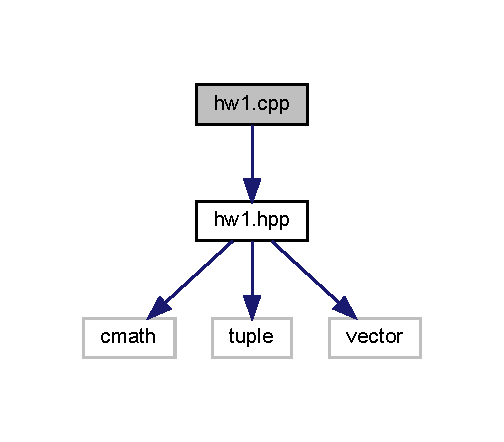
\includegraphics[width=242pt]{hw1_8cpp__incl}
\end{center}
\end{figure}
\doxysubsection*{Functions}
\begin{DoxyCompactItemize}
\item 
tuple$<$ vector$<$ double $>$, vector$<$ double $>$, vector$<$ double $>$ $>$ \mbox{\hyperlink{hw1_8cpp_a1bf4f8321c54ecf33406a82aed74d9d1}{HW1}} (double t0, double t1, int n, double y0, double y0p, double theta0)
\begin{DoxyCompactList}\small\item\em HW1\+: Solve Kepler problem via finite difference Method. \end{DoxyCompactList}\end{DoxyCompactItemize}


\doxysubsection{Detailed Description}
code for homework1 of Computer1 class in Yonsei University Use finite difference method to solve Kepler problem 

\begin{DoxyAuthor}{Author}
pistack (Junho Lee) 
\end{DoxyAuthor}
\begin{DoxyDate}{Date}
2021. 10. 10. 
\end{DoxyDate}


\doxysubsection{Function Documentation}
\mbox{\Hypertarget{hw1_8cpp_a1bf4f8321c54ecf33406a82aed74d9d1}\label{hw1_8cpp_a1bf4f8321c54ecf33406a82aed74d9d1}} 
\index{hw1.cpp@{hw1.cpp}!HW1@{HW1}}
\index{HW1@{HW1}!hw1.cpp@{hw1.cpp}}
\doxysubsubsection{\texorpdfstring{HW1()}{HW1()}}
{\footnotesize\ttfamily tuple$<$vector$<$double$>$, vector$<$double$>$, vector$<$double$>$ $>$ HW1 (\begin{DoxyParamCaption}\item[{double}]{t0,  }\item[{double}]{t1,  }\item[{int}]{n,  }\item[{double}]{y0,  }\item[{double}]{y0p,  }\item[{double}]{theta0 }\end{DoxyParamCaption})}



HW1\+: Solve Kepler problem via finite difference Method. 


\begin{DoxyParams}{Parameters}
{\em t0} & initial time \\
\hline
{\em t1} & final time \\
\hline
{\em n} & number of gird points to evaluate \\
\hline
{\em y0} & initial condition for zeta \\
\hline
{\em y0p} & intial condition for derivative of zeta \\
\hline
{\em theta0} & initial condition for theta \\
\hline
\end{DoxyParams}
\begin{DoxyReturn}{Returns}
tuple of time, zeta and theta 
\end{DoxyReturn}
\begin{DoxySeeAlso}{See also}
\mbox{\hyperlink{fdm}{Finite difference Method}} 

\mbox{\hyperlink{theta}{Theta}} 
\end{DoxySeeAlso}

\hypertarget{hw1_8hpp}{}\section{/home/lis1331/\+Documents/lecture/phy/computer/comp\+\_\+hw/\+H\+W1/src/include/hw1.hpp File Reference}
\label{hw1_8hpp}\index{/home/lis1331/\+Documents/lecture/phy/computer/comp\+\_\+hw/\+H\+W1/src/include/hw1.\+hpp@{/home/lis1331/\+Documents/lecture/phy/computer/comp\+\_\+hw/\+H\+W1/src/include/hw1.\+hpp}}


Header file for homework1 of Computer1 class in Yonsei University Use explicit Euler Method to solve Kepler problem.  


{\ttfamily \#include $<$cmath$>$}\newline
{\ttfamily \#include $<$tuple$>$}\newline
{\ttfamily \#include $<$vector$>$}\newline
Include dependency graph for hw1.\+hpp\+:\nopagebreak
\begin{figure}[H]
\begin{center}
\leavevmode
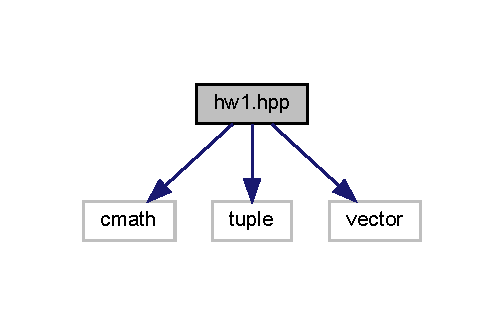
\includegraphics[width=242pt]{hw1_8hpp__incl}
\end{center}
\end{figure}
This graph shows which files directly or indirectly include this file\+:\nopagebreak
\begin{figure}[H]
\begin{center}
\leavevmode
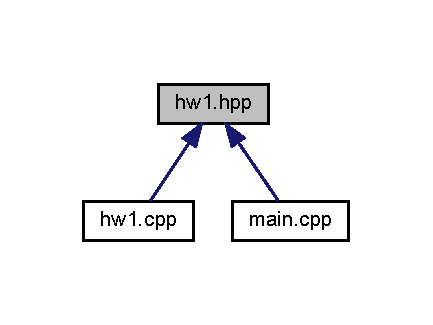
\includegraphics[width=350pt]{hw1_8hpp__dep__incl}
\end{center}
\end{figure}
\subsection*{Functions}
\begin{DoxyCompactItemize}
\item 
std\+::tuple$<$ std\+::vector$<$ double $>$, std\+::vector$<$ double $>$ $>$ \hyperlink{hw1_8hpp_ab81c50995efc39bb0b682cfb851c4ea7}{H\+W1} (double t0, double t1, int n, double y0, double y0p)
\begin{DoxyCompactList}\small\item\em H\+W1\+: Solve Kepler problem via explicit Euler Method with inital condition. \end{DoxyCompactList}\end{DoxyCompactItemize}


\subsection{Detailed Description}
Header file for homework1 of Computer1 class in Yonsei University Use explicit Euler Method to solve Kepler problem. 

\begin{DoxyAuthor}{Author}
pistack (Junho Lee) 
\end{DoxyAuthor}
\begin{DoxyDate}{Date}
2021. 10. 10. 
\end{DoxyDate}


\subsection{Function Documentation}
\mbox{\Hypertarget{hw1_8hpp_ab81c50995efc39bb0b682cfb851c4ea7}\label{hw1_8hpp_ab81c50995efc39bb0b682cfb851c4ea7}} 
\index{hw1.\+hpp@{hw1.\+hpp}!H\+W1@{H\+W1}}
\index{H\+W1@{H\+W1}!hw1.\+hpp@{hw1.\+hpp}}
\subsubsection{\texorpdfstring{H\+W1()}{HW1()}}
{\footnotesize\ttfamily std\+::tuple$<$std\+::vector$<$double$>$, std\+::vector$<$double$>$ $>$ H\+W1 (\begin{DoxyParamCaption}\item[{double}]{t0,  }\item[{double}]{t1,  }\item[{int}]{n,  }\item[{double}]{y0,  }\item[{double}]{y0p }\end{DoxyParamCaption})}



H\+W1\+: Solve Kepler problem via explicit Euler Method with inital condition. 


\begin{DoxyItemize}
\item zeta(0) = z\+\_\+0
\item zeta\textquotesingle{}(0) = z\textquotesingle{}\+\_\+0 see H\+W1.\+pdf for futher detail 
\begin{DoxyParams}{Parameters}
{\em t0} & initial time \\
\hline
{\em t1} & final time \\
\hline
{\em n} & number of gird points to evaluate \\
\hline
{\em y0} & initial condition for zeta(0) \\
\hline
{\em y0p} & intial condition for zeta\textquotesingle{}(0) \\
\hline
\end{DoxyParams}
\begin{DoxyReturn}{Returns}
tuple of time and zeta 
\end{DoxyReturn}

\end{DoxyItemize}
\hypertarget{main_8cpp}{}\section{/home/lis1331/\+Documents/lecture/phy/computer/comp\+\_\+hw/\+H\+W3/src/main.cpp File Reference}
\label{main_8cpp}\index{/home/lis1331/\+Documents/lecture/phy/computer/comp\+\_\+hw/\+H\+W3/src/main.\+cpp@{/home/lis1331/\+Documents/lecture/phy/computer/comp\+\_\+hw/\+H\+W3/src/main.\+cpp}}


main program for homework3 of Computer1 class in Yonsei University Interactively reads inital condition, number of sine function used for guess, number of gird points to evaluate, number of interation, step size and output file name then computes and saves solution.  


{\ttfamily \#include $<$string$>$}\newline
{\ttfamily \#include $<$iostream$>$}\newline
{\ttfamily \#include $<$fstream$>$}\newline
{\ttfamily \#include \char`\"{}hw3.\+hpp\char`\"{}}\newline
Include dependency graph for main.\+cpp\+:\nopagebreak
\begin{figure}[H]
\begin{center}
\leavevmode
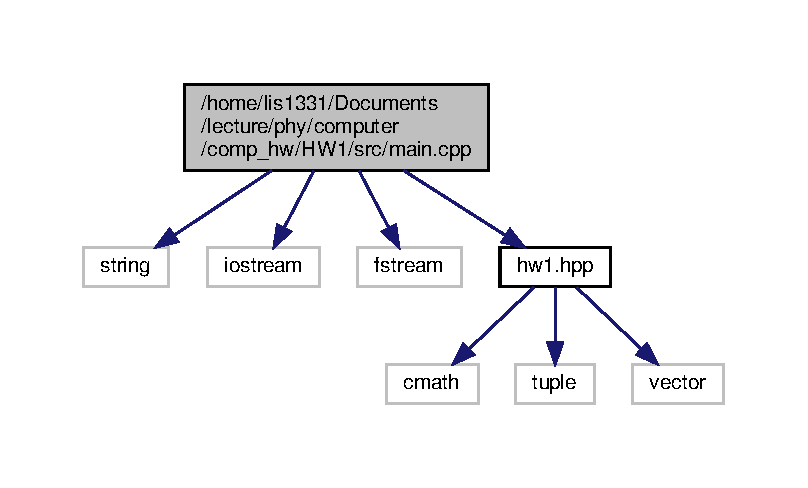
\includegraphics[width=350pt]{main_8cpp__incl}
\end{center}
\end{figure}
\subsection*{Functions}
\begin{DoxyCompactItemize}
\item 
\mbox{\Hypertarget{main_8cpp_a840291bc02cba5474a4cb46a9b9566fe}\label{main_8cpp_a840291bc02cba5474a4cb46a9b9566fe}} 
int {\bfseries main} (void)
\end{DoxyCompactItemize}


\subsection{Detailed Description}
main program for homework3 of Computer1 class in Yonsei University Interactively reads inital condition, number of sine function used for guess, number of gird points to evaluate, number of interation, step size and output file name then computes and saves solution. 

\begin{DoxyAuthor}{Author}
pistack (Junho Lee) 
\end{DoxyAuthor}
\begin{DoxyDate}{Date}
2021. 10. 10. 
\end{DoxyDate}

%--- End generated contents ---

% Index
\backmatter
\newpage
\phantomsection
\clearemptydoublepage
\addcontentsline{toc}{chapter}{Index}
\printindex

\end{document}
